
\chapter{One Dimensional gas dynamics}\label{chap2}

\section{Equations of motion}\label{chap2:sec2.1}

These\pageoriginale equations of motion completely characterise smooth movement of a fluid. They express the physical laws:
\begin{itemize}
\item[{\rm i)}] Conservation of mass,

\item[{\rm ii)}] Conservation of momentum and 

\item[{\rm iii)}] Conservation of energy.
\end{itemize}

We first consider conservation of mass. For this, the rate of change of mass in any volume element $V$ of the fluid is balanced by the flow across $\partial V$, the boundary of $V$. If $\u{n}$ denotes the outward unit normal to $\partial V$, then the normal component of velocity across $\partial V$ is $\u{n} \cdot \u{u}$, where $\u{u} = (u_1, u_2, u_3)$ is the velocity vector of the fluid (we are mainly interested in 1, 2 or 3 dimensional flows). Then the net flow across the boundary between two times $t_1, t_2$ is 
$$
- \int\limits^{t_2}_{t_1} \int\limits_{\partial V} \rho (\u{n} \cdot \u{u}) d \sigma dt,
$$
where $\rho$ is the density of the fluid and $d\sigma$ denotes the surface measure. This must be balanced by the change in total mass between the times $t_1$, $t_2$. Hence
$$
[\int\limits_V \rho d V]^{t_2}_{t_1}  =  - \int\limits^{t_2}_{t_1} \int\limits_{\partial V} \rho (\u{n} \cdot \u{u}) d \sigma \; dt, 
$$
or taking the limit as $t_1 \to t_2$, 
$$
\frac{d}{dt} \int\limits_V \rho d V + \int\limits_{\partial V} \rho (\u{n} \cdot \u{u}) d \sigma = 0. 
$$
Using\pageoriginale divergence theorem this can be written as
\begin{equation*}
\frac{d}{dt} \int\limits_V \rho d V + \int\limits_V \divv (\rho \u{u}) d V = 0.
\tag{2.1}\label{eq2.1}
\end{equation*}
In a similar way, the equation for the net change in the $i^{\rm th}$ component of the momentum is 
\begin{equation*}
\frac{d}{dt} \int\limits_V \rho u_i d V + \int\limits_{\partial V} [\rho u_i (\u{n} \cdot \u{u}) + pn_i] d\sigma = 0. \tag{2.2}\label{eq2.2}
\end{equation*}
The first term is the rate of change of total momentum inside $V$, the second term is the transport of the momentum across the boundary and the third is the rate of change of momentum produced by the pressure  $p$. Here, we are neglecting other forces such as gravity, viscosity, etc.

The total energy density per unit volume consists of the kinetic energy $\rho |\u{u}|^2 /2$ of the motion of particles plus the internal energy $\rho e$ of the molecular motion. For energy balance, we then have after neglecting heat conduction, viscosity, etc. 
\begin{equation*}
\frac{d}{dt} \int\limits_V (\rho |\u{u}|^2 / 2 + \rho e) dV + \int\limits_{\partial V} \{(\rho |\u{u}|^2 + \rho e) \u{n} \cdot \u{u} + p \u{n} \cdot \u{u} \}  d \sigma = 0. 
\tag{2.3}\label{eq2.3}
\end{equation*}
The first term in the surface integral is again the contribution from energy transport across the  boundary and the second term is the rate of work by the pressure $p$ at the boundary.

If discontinuities are allowed in the flow, we have to work with (\ref{eq2.1}) - (\ref{eq2.3}) (In fact they are not quite enough). But if all the quantities are smooth, we can different under the integral sign. We then obtain the differential equations
\begin{align*}
& \frac{\partial \rho}{\partial t} + \divv (\rho \u{u}) = 0, \tag{2.1(a)}\label{eq2.1a}\\
& \frac{\partial}{\partial t} (\rho u_i) + \divv (\rho u_i \u{u}) + \frac{\partial p}{\partial x_i} = 0,\quad i = 1,2,3, \tag{2.2(a)}\label{eq2.2a}\\
& \frac{\partial}{\partial t} (\rho |\u{u}|^2 / 2 + \rho e) + \divv [\rho \u{u} (\rho |\u{u}|^2 / 2 + e + \frac{p}{\rho})] = 0. \tag{2.3(a)}\label{eq2.3a}
\end{align*}\pageoriginale

\section{Thermodynamical relations. Entropy:}\label{chap2:sec2.2}

Consider the quantity $de + pd (1/\rho)$. When a small energy is added to a mass of gas some of the energy is the work of changing the volume $1/\rho$ to $1/\rho + d (1/\rho)$. This energy is $pd(1/\rho)$; the rest $de$ is heat put into the system. Since the quantity $de$ is a perfect differential, there exist functions $S(p,\rho)$, $T(p,\rho)$ such that 
\begin{equation*}
de + pd (1/\rho) = TdS
\tag{2.4}\label{eq2.4}
\end{equation*}
$T$ is the absolute temperature and $S$ is the entropy. The relation (\ref{eq2.4}) may be viewed as a way of defining temperature and entropy up to an arbitrary function.

Suppose we treat $p$, $\tau = \rho^{-1}$ as the independent variables, then we will have
$$
de = - pd\tau + \alpha d p + \beta d \tau,
$$
where $\alpha, \beta$ are given functions and we want to express $\alpha d p + \beta d \tau$ as $T dS$, where $T,S$ are functions of $p,\tau$. We want to show this representation is essentially unique. First from the compatibility relations for $de$, we have
\begin{equation*}
(-p + \beta)_p = \alpha_\tau,
\tag*{$(\ast)$}
\end{equation*}
and from\pageoriginale the one for $S$ we have
$$
(\alpha/ T)_\tau = (\beta/T)_p
$$
or 
$$
\alpha (\frac{1}{T})_\tau -\beta (\frac{1}{T})_p + (\alpha_\tau - \beta_p) \frac{1}{T} = 0 
$$
or 
$$
\alpha (\frac{1}{T})_\tau - \beta (\frac{1}{T})_p - \frac{1}{T} = 0, \quad \text{from $(\ast)$}. 
$$
This is a first order equation for $1/T$ which we may solve provided $a^2 + \beta^2 \neq 0$, which is a reasonable thermodynamic assumption. Once $T$ is determined $S$ is found from $dS = (\alpha / T) dp + (\beta / T) d\tau$. With respect to uniqueness, suppose we have two such representations, $T,S$ and $T', S'$. Then $TdS = T' dS'$ or $S_\tau/S_p = S'_\tau / S'_p$ and hence $F(S,S') = 0$ for some $F$ or with an assumption of monotonicity $S' = s(S)$ and then $T' = \dfrac{T}{ds/dS}$. Thus the temperature and entropy are uniquely determined up to a scaling factor $s(S)$.

Suppose, we know for some medium that $e$ is a function of $\tau$ and $S$, where $\tau = 1/ \rho$, specific volume. Then we see that $p$ is also a function of $\rho$, $S$. We assume 
$$
p = f(\rho, S) \quad \text{or} \quad  p = g(\tau, S). 
$$
It is a fundamental property of almost all media that, entropy remaining constant, pressure is an increasing function of $\rho$ or equivalently decreasing function of $\tau$. Thus
$$
f_\rho > 0 \quad \text{and} \quad g_\tau < 0. 
$$
For any value of $S$, the function $g(\tau, S)$ is generally convex\pageoriginale w.r.t. $\tau$. Henceforth, we shall assume this:
$$
g_{\tau\tau} (r,S) >0.
$$

\medskip
\noindent{\textbf{Alternative forms of equations of motion: }}

Introducing the operator
$$
\frac{D}{Dt} = \frac{\partial}{\partial t} + u_j \cdot \frac{\partial}{\partial x_j}, 
$$
the equations (\ref{eq2.1a}) - (\ref{eq2.3a}) can be written as
\begin{align*}
& \frac{D\rho}{Dt} + \frac{\partial u_j}{\partial x_j} = 0, \tag{2.5}\label{eq2.5}\\
\rho & \frac{Du_i}{Dt} + \frac{\partial p}{\partial x_i} = 0, \quad i = 1,2,3, \tag{2.6}\label{eq2.6}\\
\rho & \frac{De}{Dt} + p \cdot \frac{\partial u_j}{\partial x_j} = 0, \tag{2.7}\label{eq2.7}
\end{align*}
or using (\ref{eq2.5}), (\ref{eq2.7}) can be written as 
$$
\frac{De}{Dt} - \frac{p}{\rho^2} \; \frac{D\rho}{Dt} = 0.
$$
Then from the thermodynamic relation (\ref{eq2.4}), we obtain
\begin{equation*}
T \frac{DS}{Dt} = 0. \tag{2.8}\label{eq2.8}
\end{equation*}
This is to say, entropy remains constant following a particle. Flows satisfying (\ref{eq2.8}) are called {\em adiabatic}. It follows from that, if the fluid initially has uniform entropy then entropy remains constant throughout as long as the flow is continuous. In such  a case $p = f(\rho)$. Such flows are called {\em isentropic}. 

\section{One dimensional flow}\label{chap2:sec2.3}

The equations reduce to 
\begin{equation*}
\left. 
\begin{aligned}
& \rho_t + (\rho u)_x = 0,\\
& (\rho u )_t + (\rho u^2)_x + p_x = 0, \\
& S_t + uS_x = 0. 
\end{aligned}
\right\} \tag{2.9}\label{eq2.9}
\end{equation*}\pageoriginale
The second equation in (\ref{eq2.9}) can be written, using the first equation, as 
$$
\rho u_t + \rho u u_x + p_x = 0.
$$
The third equation follows from (\ref{eq2.8}). It is convenient to use $p$, $u$. Then the system (\ref{eq2.9}) may be written as
\begin{align*}
& p_t + up_x + \rho c^2 u_x = 0, \\
& \rho u_t + p_x + \rho u u_x = 0, \tag{2.9(a)}\label{eq2.9a}\\
& S_t + uS_x = 0, 
\end{align*}
where $c^2 = (\partial p / \partial \rho)_{S =  \text{ constant}}$; $c$ is called the sound speed. System (\ref{eq2.9a}) is a typical nonlinear hyperbolic system.

Another such ta system, the Lundquist equations, occurs in magneto-hydrodynamics. It involves coupling Maxwell's equations with the classical equations of gas dynamics.

Let $E,B$ stand for electric and magnetic field vectors and let $J$, $u$ denote the electric current and the flow velocity. If $p$ is pressure and $c^2 = dp/d\rho$ is the sound velocity, then the equations are
\begin{align*}
& \frac{\partial B}{\partial t} + (\nabla \cdot u) B - (B \cdot \nabla) u = 0, \\
\rho & \frac{\partial u}{\partial t} + \nabla p + B \times (\nabla \times B) = 0,\\
& c^2 / \rho \cdot \frac{\partial \rho }{\partial t} + c^2 \nabla \cdot u = 0,\\
& \frac{dS}{dt} = 0.
\end{align*}
Another\pageoriginale related hyperbolic system occurs in the theory of shallow water where (\ref{eq2.5}) and (\ref{eq2.6}) hold  with the depth playing the role of density $\rho$ and $p/\rho^2$ is constant.

We turn to the study of the system (\ref{eq2.9a}). We consider isentropic flow so that the third equation drops out. Adding and substracting the other two equations, we arrive at
\begin{align*}
& p_t + (u+c) p_x + \rho c \{u_t + (u+c) u_x\} =0,\\
& p_t + (u-c)p_x - \rho c \{u_t + (u-c) u_x\} = 0.
\end{align*}
We choose the characteristics $C_+$, $C_-$ so that the derivatives are along them. Thus for 
\begin{align*}
 C_+ : \frac{dx}{dt} & = u + c, \\
 C_- : \frac{dx}{dt} & = u - c
\end{align*}
and then
\begin{align*}
\frac{dp}{dt} + \rho c \frac{du}{dt} & = 0 \quad \text{on} \quad C_+\\
\frac{dp}{dt} - \rho c \frac{du}{dt} & = 0 \quad \text{on} \quad C_-.
\end{align*}
Integrating these two equations, we obtain
\begin{align*}
 \ell (\rho) + u & = \text{ constant on } C_+,\\
 \ell (\rho) - u & = \text{ constant on } C_-,
\end{align*} 
where 
$$
\ell (\rho) = \int \frac{c(\rho) d\rho}{\rho}
$$
The quantities $\ell (\rho) \pm u$ are called {\em Riemann invariants}.

\begin{exercise}\label{chap2:exer2.1}
Reduce\pageoriginale the system (\ref{eq2.9a}) (omitting the last equation) for slow speeds nearly constant  density to the wave equation (in $u$ or in $p$). Show also that discontinuities in derivatives propagate with sound speed.
\end{exercise}

\begin{exercise}\label{chap2:exer2.2}
Find the speeds of propagation of the one dimensional Lundquist equations.
\end{exercise}

\medskip
\noindent{\textbf{Simple Waves. Piston Problem: }}
In addition to being isentropic, if the flow has one Riemann invariant constant throughout, the solution is called a {\em simple wave}. Such a wave lies next to a constant state since all the characteristics of one kind issuing from the constant state carry a constant Riemann invariant. 

To illustrate, how such waves can be produced, we consider the piston problem as a basic model. Consider the waves produced by the movement of a piston at the end of a tube and gas at rest in a constant state ahead of it. Provided shocks do not appear, the waves carry a constant Riemann invariant from the constant state ahead.

Initially, the gas has velocity $u=0$, sound speed $c_o$ and $S= S_o$ in $s \geq 0$, $t=0$. The piston path is itself a particle path and the flow is isentropic.

Since $u- c< u$ the $C_-$ characteristics start on the $x$ - axis in the uniform region (see figure 2.1). On each $C_-$
\begin{equation*}
\ell (\rho) - u = \text{ constant;}\tag{2.10}\label{eq2.10}
\end{equation*}
Since\pageoriginale $u=0$ initially, we conclude that the constant is $\ell(\rho_0)$, where $\rho_0$ corresponds to the initial density. Since this constant is the same for $C_-$ characteristics, we conclude that $\ell(\rho) - u$ is the Riemann invariant that is constant throughout. We now use the other characteristic to find the other quantities. 
\begin{figure}[H]
\centering
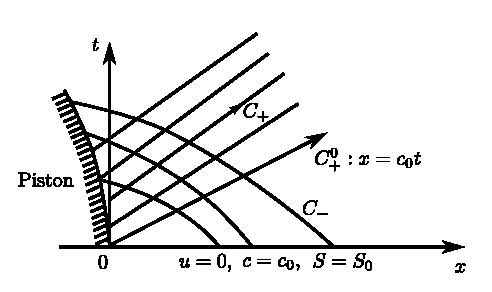
\includegraphics{figures/fig2.1.eps}
\centerline{\bf Fig. 2.1.}
\end{figure}

For those $C_+$ which originate from the $x$-axis, we see that
\begin{equation*}
\ell (\rho) + u = \ell (\rho_0)\tag{2.11}\label{eq2.11}
\end{equation*}
From (\ref{eq2.10}), (\ref{eq2.11}), we conclude that $u=0$, $c = c_0$ in the region covered by these $C_+$ characteristics. Let $C^o_+$ separate the $C_+$ characteristics that meet the piston from those which meet the $x$ - axis.

Since the image of the flow in $(\rho, u)$ space lies entirely on the curve $\ell'(\rho) - u = $ constant each point on the curve represents a curve in the flow. At that point the value of $\ell (\rho ) + u$ determines $u,\rho$ and hence the slope $dx/dt = u + c$,  of $C_+$ which is constant along that characteristic. Hence

$\rho$, $u$ are constant on each $C_+ : \dfrac{dx}{dt} = u + c$. 

To complete\pageoriginale the solution, we should use the boundary conditions, given on the piston. Let the piston path be given by $x = X(t)$. Then the boundary condition is 
$$
u = \dot{X}(t) \quad \text{on} \quad x = X(t).
$$
With this, we can obtain the complete solution:
\begin{align*}
 x & = (\dot{X} (\tau) + c) \; (t-\tau)\\
 u & = \dot{X} (\tau)
\end{align*}

Since the $C_+$ characteristics are straight lines with the slope $dx/dt$ increasing with $u$, it is clear that the characteristics will overlap if $u$ increases on the piston i.e., if $\ddot{X}(t) > 0$ for any $t$ (this is the case when the piston accelerates into the gas). This is typical of nonlinear breaking, (see p8) and shocks will be formed. We need to reexamine the arguments leading to the constancy of entropy and of one of the Riemann invariants. But for motions with $\ddot{X}(t) \leq 0$, we have constructed a complete solution.

\section{Shock conditions}\label{chap2:sec2.4}

We suppose the flow is one dimensional and allow jump discontinuities, denoted by $[\cdot]$, in the flow. We must work with the equations (\ref{eq2.1}) - (\ref{eq2.3}). Let the region $V$ collapse on a slit around the discontinuity and we find the discontinuity conditions:
\begin{gather*}
- U[\rho] + [\rho u] = 0\\
- U[\rho u] + [\rho u^2 + p] = 0\\
- U [\rho^2 / 2 + \rho e] + [(\rho u^2 / 2 + \rho e + p) u] = 0,  
\end{gather*}
where $U$ is\pageoriginale the discontinuity velocity. We denote by subscripts (0), (1) the two states. As a particle moves across the discontinuity, it moves from the {\em front} of the discontinuity across the discontinuity to {\em behind} the discontinuity. The entropy must {\em increase} in this direction.

For convenience, we introduce the relative velocities
$$
v_i = U - u_i, \quad i = 0,1.
$$
In the velocity frame where the discontinuity is at rest, since the equations are independent of the coordinate system, we obtain from the above
\begin{equation*}
\rho_0 v_0 = \rho_1 v_1 = m, \tag{2.12}\label{eq2.12}
\end{equation*}
where $m$ is the {\em mass flux } through the surface;
\begin{equation*}
\rho_0 v^2_0 + p_0 = \rho_1 v^2_1 + p_1 = p, 
\tag{2.13}\label{eq2.13}
\end{equation*}
where $p$ is total {\em momentum flux} and finally the {\em energy flux} condition:
\begin{equation*}
m(v^2_0/2 + e_0 + p_0 \tau_0) = m (v^2_1 /2 + e_1+p_1 \tau_1). 
\tag{2.14}\label{eq2.14}
\end{equation*}
According to the second law of thermodynamics entropy can only increase. Hence across a discontinuity
$$
S_0 \leq S_1
$$ 
or
\begin{equation*}
mS_0 \leq mS_1\tag{2.15}\label{eq2.15}
\end{equation*}
Two two types of discontinuity surfaces are distinguished by  the cases $m = 0$ and $m \neq 0$. The case $m \neq 0$ corresponds to mass flowing across and the discontinuity surfaces are called\pageoriginale {\em check} fronts; the case $m=0$ corresponds to a {\em contact} or {\em slip} surface.

We first consider the case of a shock, $m \neq 0$. Then from equation (\ref{eq2.14}), we obtain 
$$
\frac{1}{2} v^2_0 + e_0  + p_0 \tau_0 = \frac{1}{2} v^2_1 + e_1 + p_1 \tau_1.  
$$

If we introduce {\em enthalpy}, $i=e+p\tau$, we then obtain
\begin{equation*} 
v^2_0 / 2 + i_0 = v^2_1/ 2 + i_1 
\tag{2.16}\label{eq2.16}
\end{equation*}
If we use (\ref{eq2.12}) and (\ref{eq2.13}), we obtain
\begin{align*}
\tau_0 (p_0 - p_1) & = v_0 (v_1 - v_0),\\
\tau_1 (p_0 - p_1) & = v_1 (v_1 - v_0)
\end{align*}
and hence adding these two equations, we obtain
\begin{equation*}
(\tau_0 + \tau_1) \; (p_1 - p_0) = v^2_0 - v^2_1\tag{2.17}\label{eq2.17}
\end{equation*}
Equation (\ref{eq2.16}) becomes
\begin{equation*}
(p_1 - p_0) \; ( \tau_0 + \tau_1) / 2 = i_1 - i_0, 
\tag{2.18}\label{eq2.18}
\end{equation*}
or, since $i=e+p\tau$,
\begin{equation*}
(\tau_0 - \tau_1) \; (p_1 + p_0) / 2 = e_1 - e_0. 
\tag{2.19}\label{eq2.19}
\end{equation*}
Since (\ref{eq2.18}) and (\ref{eq2.19}) involve only thermodynamical quantities, they are particularly useful. They were first studied by Hugoniot and (\ref{eq2.19}) is called the {\em Hugoniot relation}. The relation (\ref{eq2.19}) can be intepreted by stating that the increase in energy across a shock is due to the work done by the mean of the pressures in performing the {\em compression.}

The most\pageoriginale common example considered is a polytropic gas, with $p = A (S)\rho^\gamma$. We note the following relations: (refer Serrin\footnote{See, Fl\"ugge, S. (Ed.), Encyclopedia of Physics, VIII/1, Springer--Verlag (1959).})
$$
\log A = S/c_\nu, \quad e = p / (\gamma - 1) \rho, \quad c^2 = \gamma p / \rho, 
$$
where $c_\nu$ is the specific heat at constant volume. It is often useful to use formulas for polytropic gases with the parameter 
$$
M = \frac{U - u_0}{c_0}
$$
which is the {\em Mach number} of the shock relative to the flow ahead and is a useful measure of strength. Using (\ref{eq2.12}) and (\ref{eq2.13}) and the definition of $M$, we arrive at the following:
\begin{align*}
& |\frac{u_1 - u_0}{c_0}| = \frac{2(M^2 - 1)}{(\gamma +1)M}, \\
& \rho_1 / \rho_0 = (\gamma + 1) M^2 / \{(\gamma - 1) M^2 + 2\},\\
& (p_1 - p_0) / p_0 = 2 \gamma (M^2 -1) / (\gamma +1),\\
& c_1 / c_0 = \frac{\{2 \gamma M^2 - (\gamma -1)\}^{1/2} \cdot \{(\gamma -1) M^2 + 2\}^{1/2}}{(\gamma + 1)M}.
\end{align*}
Introducing an alternative strength parameter
$$
z = \frac{p_1 - p_0}{p_0}, 
$$
the above set of equations can be written as 
\begin{align*}
& M = \left\{1+\frac{(\gamma + 1)z}{2\gamma} \right\}^{1/2},
\tag{2.20}\label{eq2.20}\\
& |\frac{u_1 - u_0}{c_0}| = \frac{z}{\gamma \{1 + \frac{(\gamma +1)z}{2\gamma}\}^{1/2}}, \tag{2.21}\label{eq2.21}\\
& \rho_1 / \rho_0 =  \left\{1+ \frac{(\gamma + 1)z}{2\gamma} \right\} / \left\{1+ \frac{(\gamma -1)z}{2\gamma}  \right\}, \tag{2.22}\label{eq2.22}\\
& c_1 / c_0 = \left\{\frac{(1+z) (1+ \frac{(\gamma -1)z}{2\gamma})}{1+\frac{(\gamma + 1)z}{2\gamma}} \right\}^{1/2} \tag{2.23}\label{eq2.23}
\end{align*}\pageoriginale 
From the relation for $S$, obtained from $A$, and the relation (\ref{eq2.22}), we obtain
\begin{equation*}
(S_1 - S_0) / c_\nu = \log \left\{ \frac{(1+z) (1+ \frac{(\gamma -1)}{2\gamma})z}{(1+\frac{(\gamma +1)}{2\gamma} z)\gamma}\right\} \tag{2.24}\label{eq2.24}
\end{equation*}
Since $S_1 > S_0$ across a shock, we obtain, as is easily seen by expanding that $z>0$. Hence $p_1 > p_0$, and from the above relations, we then obtain
$$
\rho_1 > \rho_0 , \; c_1 > c_0, \; u_1 > u_0, \; M>1. 
$$
From (\ref{eq2.20}), it is clear that $U> u_0+c_0$. From the relations (\ref{eq2.20}), (\ref{eq2.21}) and (\ref{eq2.23}), it then follows that,
$$
u_1 + c_1 > U.
$$
Thus a polytropic shock is always compressive with $p_1>p_0$ and it is supersonic viewed from ahead and subsonic from behind.

These facts are true quite generally, but we will discuss this later, when we study the Riemann problem.

\section{Contact Discontinuities}\label{chap2:sec2.5}
If the mass flux $m$ through the surface of discontinuity is zero, then $v_1= v_0 = 0$, so that\pageoriginale $u_1 = u_0 = U$. Then we have $p_0 = p_1$ from (\ref{eq2.13}) and (\ref{eq2.14}) is automatically satisfied. Such a discontinuity surface as indicated before, is called a {\em contact} or {\em slip surface}.

The flow velocity is continuous across the contact surfaces in one dimensional flow, but in higher dimensions the tangential component of the velocity vector may suffer a discontinuity across a contact surface, while the normal component relative to the surface is always zero. For details see, e.g., Courant--Friedrichs \cite{key6}.

\section{Shock Reflection}\label{chap2:sec2.6}
A simple example of determining a flow with shocks is provided by the reflection of a shock from a wall which can also be solved exactly. A shock with a state behind of prescribed velocity hits a wall and is reflected. We seek the pressure after reflection.

Let the subscripts $0,1$ refer to the states ahead of and behind the incident shock, and subscript 2 refer to the state behind the reflected shock, see figure 2.2.
\newpage

\begin{figure}[H]
\centering
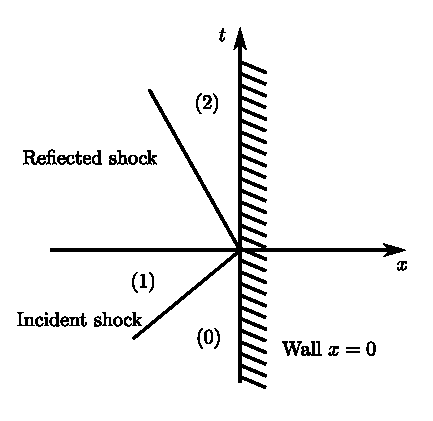
\includegraphics{figures/fig2.2.eps}
\centerline{\bf Fig. 2.2.}
\end{figure}


If the\pageoriginale shock strength of the incident shock is $z_I = (p_1 - p_0)/ p_0$, the state (1) can be determined by the relations (\ref{eq2.20}) - (\ref{eq2.24}). If
$$
z_R = (p_2 - p_1)/p_1
$$
is the strength of the reflected shock, we obtain, with suitable change in the sign of the velocities since the reflected shock travels in the opposite direction to the incoming shock, from (\ref{eq2.21}) that
$$
|\frac{u_1 - u_2}{c_1}| = \frac{z_R}{\gamma \left\{1+\frac{(\gamma + 1)z_R}{2\gamma}  \right\}^{1/2}}.
$$
Next to the wall, the gas must be at rest and hence $u_2 = u_0 = 0$. Now, $u_1$ and $c_1$ can be found in terms of $z_I$. After doing this, we obtain
$$
\frac{z_I}{\gamma\{(1+z_I) \; (1+\frac{(\gamma - Iz_I)}{2\gamma})\}^{1/2}} = \frac{z_R}{ \gamma \{1+\frac{(\gamma + 1)z_R}{2\gamma}\}^{1/2}}
$$
This is a quadratic in $z_R$ and it is easily seen that the relevant solution is 
$$
z_R = \frac{z_I}{1 + \frac{(\gamma -1)z_I}{2\gamma}}
$$
For weak shocks $z_I \to 0$ and hence $z_R \simeq z_I$ and 
$$
p_2 - p_0 \simeq 2 (p_1 - p_0). 
$$
So, for\pageoriginale the acoustic case, the pressure is doubled as is well known. Also for strong shocks $z_I \to \infty$. This implies $z_R = \dfrac{2\gamma}{(\gamma -1)}$ and therefore
$$
\frac{p_2}{p_1} \quad \frac{3\gamma -1}{\gamma -1} = 8
$$
for $\gamma = 1.4$. Hence there is a large gain in pressure after reflection. This phenomenon is even more striking in spherically symmetric flows when a shock is reflected at the center of symmetry.

\section{Hugoniot Curve. Shock Determinacy}\label{chap2:sec2.7}
We recall the Hugoniot relation (\ref{eq2.19}):
$$
e_1 - e_0 = (\tau_0 - \tau_1) \; (p_1 + p_0 ) /2.
$$
We regard all quantities such as energy $e$, entropy $S$ etc. as functions of $\tau, p$. We define the {\em Hugoniot function}
$$
H(\tau, p) = e(\tau, p) - e(\tau_0 - p_0) + (\tau - \tau_0) \; (p+p_0) /2. 
$$
If $(\tau_0 , p_0)$ is fixed, the graph of the points $(\tau, p)$ which satisfy $H(\tau, p) = 0$ is the {\em Hugoniot curve}. As we shall see with $p>p_0$ it represents all possible states that can be reached with $(\tau_0, p_0)$ ahead of the {\em shock}. For $p<p_0$ the curve represents the states that can be ahead of $(\tau_0, p_0)$. The big advantage in considering this curve is that it involves no velocities.

For polytropic gases, we have 
$$
e = \frac{p\tau}{(\gamma -1)} = \frac{p\tau (1-\mu^2)}{2\mu^2},
$$
where\pageoriginale
$$
\mu^2 = \frac{(\gamma -1)}{(\gamma + 1)}. 
$$
Hence
$$
2\mu^2 H(\tau, p) = (\tau - \mu^2 \tau_0) p - (\tau_0 - \mu^2 \tau) p_0.
$$
Hence the Hugoniot curve, specifically the Hugoniot curve with center $(\tau_0, p_0)$, is a rectangular hyperbola with the left asymptote
$$
\tau = \mu^2 \tau_0= \tau_{\rm min} > 0.
$$
(See figure 2.3)
\begin{figure}[H]
\centering
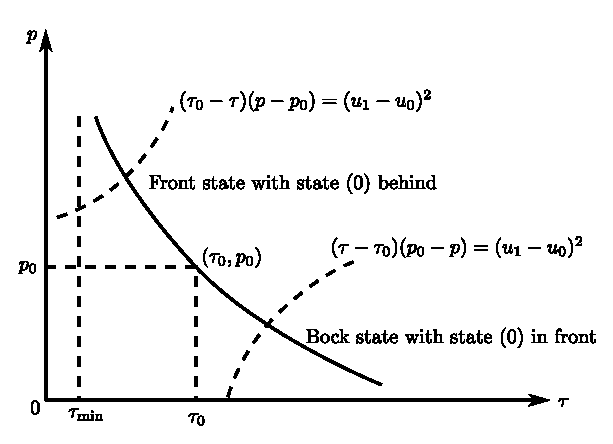
\includegraphics{figures/fig2.3.eps}
\centerline{\textbf{Fig. 2.3.} The Hugoniot curve is the heavy curve.}
\end{figure}

We shall see that under wide conditions on the Hugoniot curve the state $(\tau, p)$ that can lie ahead or behind $(\tau_0, p_0)$ and connected by a shock, can be found exactly.

The precise\pageoriginale statements are:
\begin{enumerate}
\item The state (0), i.e., in which $(\tau_0, p_0)$ is given, and the shock velocity $U$ determine the complete state (1) on the other side of the shock front.

\item The state (0) and the velocity $u_1$ determine the speed of the shock front and the complete state (1) if it is specified whether the state (0) should be ahead of or behind the shock front.

\item The state (0) and the pressure $p_1$ determine the speed of the shock front and the complete state (1).
\end{enumerate}

To prove these statements, we make the following assumptions on the Hugoniot curve $H(\tau, p) = 0$ with center $(\tau_0, p_0)$:
\begin{itemize}
\item[{\rm (H1)}] Along the Hugoniot curve, the pressure varies from zero to infinity and the value of $\tau$ exceeds $\tau_{\min}$.

\item[{\rm (H2)}] The Hugoniot curve is strictly decreasing, i.e. $\dfrac{dp}{d\tau} < 0$ along the curve.

\item[{\rm (H3)}] Every ray through $(\tau_0, p_0)$ intersects the Hugoniot curve at exactly one point and at $(\tau_0, p_0)$, $\dfrac{d^2 p}{d\tau^2} >0$.
\end{itemize}

(All three conditions are satisfied by the polytropic gases).

We are now in a position to prove statements (1) - (3) made above provided {\em we assume pressure increases across a shock}. It follows from the shock condition (\ref{eq2.12}) and (\ref{eq2.13}) that 
\begin{equation*}
- m^2 = p^2_0 v^2_0 = \frac{p_1 - p_0}{\tau_1 - \tau_0}
\tag{2.25}\label{eq2.25}
\end{equation*}
So, to find $(\tau_1, p_1)$, we need to find the intersection of the curve\pageoriginale with the  line through $(\tau_0, p_n)$ and with slope $-m^2$. Then (H3) assumes there is just one such intersection. The velocity $u_1$ can then be found through (\ref{eq2.12}), $u_1 = U - m\tau_1$. This proves statement (1). 

As far as second statement is concerned, it can be easily derived from (\ref{eq2.12}) and (\ref{eq2.13}) that 
\begin{equation*}
-(\tau_0 - \tau_1) \; (p_0 - p_1) = (v_1 - v_0)^2. \tag{2.26}\label{eq2.26}
\end{equation*}
From the data given, $(u_1 - u_0)^2 = (v_1 - v_0)^2$, is known. Hence to find $(\tau_1, p_1)$ it suffices to find the intersection of the hyperbola
$$
(\tau_0 - \tau) \; (p_0 - p) = - (v_1 - v_0)^2
$$
with the Hugoniot curve. The slope of the hyperbola is $m^2 > 0$. Hence from (H2), it follows that there are just two such intersections, corresponding to the two possibilities that the state (0) lies ahead of or behind the shock front (see figure 2.3). The shock velocity and the state (1) can then be found easily using shock conditions. 

To prove statement (3), assume the state (0) and $p_1$ are given. The assumptions (H1)
 and (H2) assert that there is exactly one $\tau_1$ such that $H(\tau_1, p_1) = 0$. The other quantities to determine the state (1) completely are then found essentially as above.

We shall discuss a few more qualitative statements about the shock transition using the Hugoniot relation; in particular, some of the properties of the shock transistion were already\pageoriginale discussed  in an earlier section for polytropic gases. The main thing we are going to prove here is the following:
\begin{center}
\begin{quote}
\textit{The increase of entropy across a shock is}\\
\textit{of the third order in the shock strength}\\
\textit{and the shock is compressive.}
\end{quote}
\end{center}
By the shock strength, here, we mean one of the quantitites
$$
\rho_1 - \rho_0, \quad p_1 - p_0, \quad \text{or} \quad |v_1 - v_0|. 
$$

We can consider, because of (H2), the Hugoniot curve as $p = G(\tau)$; in particular, we can consider $\tau$ as independent variable. Now along the Hugoniot curve $dH=0$. So,
$$
2de + (\tau - \tau_0) dp + (p-p_0) d\tau = 0. 
$$
But $de + pd\tau = TdS$ and therefore we obtain
\begin{equation*}
2TdS - (p-p_0) d\tau  + (\tau - \tau_0) dp = 0
\tag{2.27}\label{eq2.27}
\end{equation*}
and hence
\begin{equation*}
dS = 0 \quad \text{at} \quad (\tau_0, p_0), \quad \text{the center}. \tag{2.28}\label{eq2.28}
\end{equation*}
Differentiating (\ref{eq2.27}), we obtain
\begin{equation*}
2d (TdS) +(\tau - \tau_0) d^2 p =0,\tag{2.29}\label{eq2.29}
\end{equation*}
and hence again at the center $(\tau_0, p_0)$
$$
d(TdS) = dTdS + Td^2 S = 0
$$
and therefore from (\ref{eq2.28})
$$
d^2 S = 0.
$$
Thus the\pageoriginale change in entropy is at least of third order. We show it is of third order. Differentiating (\ref{eq2.29}), we obtain, at the center $(\tau_0, p_0)$,
$$
2Td^3 S + d \tau d^2p =0.
$$
Thus since $d^2 p/d\tau^2 >0$ at $(\tau_0, p_0)$, we have
$$
d^3 S \gtrless 0 \quad \text{if} \quad d\tau \lessgtr 0 \quad \text{at} \quad (\tau_0, p_0)
$$
which proves entropy change is of third order exactly.

Furthermore, since the entropy must increase, we must have $d\tau < 0$ which means the shock is compressive and hence the upper branch of the Hugoniot curve represents states behind the state $(\tau_0, p_0)$ as was asserted earlier.

\begin{exer*}
\textbf{Piston at uniform speed: } It is a simple exercise to find the flow if a piston is moved with uniform speed {\em into} a gas at rest. The speed of the flow behind the shock is that of the piston and so we are in case 2. 
\end{exer*}

\begin{remark*}
We need the notion of vorticity in three dimensions. The vorticity is defined by
$$
\u{\omega} = \text{ curl } \u{u}.
$$
\end{remark*}

\begin{claim*}
The change in vorticity across a shock is also of third order. In a steady flow the vorticity vector $\u{\omega}$ and velocity vector $\u{u}$ satisfy
$$
\nabla (|\u{u}|^2/2) + (\u{\omega} \times \u{u}) + \frac{1}{\rho} \nabla p = \text{ constant.}
$$
Note that if $\u{\omega} \equiv 0$, i.e., if the flow is irrotational, we have Bernoulli's law. Taking a scalar product with a vector $\xi,|\xi| = 1$,\pageoriginale lying in the shock surface and letting $[\cdot]$ to denote difference across the shock, we have
$$
[\frac{d}{ds} (|\u{u}|^2 / 2 + p / \rho) - p \frac{d}{ds} (1/\rho)] - [\xi \cdot (\u{u} \times \u{\omega})] = 0, 
$$
where the differentiation w.r.t. arc length along the shock is denoted by $d/ds$; but since
$$
[|u|^2 / 2 + p/ \rho] = - [e]
$$
and 
$$
de + pd (1/\rho) = TdS,
$$
we obtain
$$
[T \frac{dS}{ds}] = [\u{\omega} \cdot (\u{\xi} \times \u{u})]. 
$$
Thus the change in $\u{\omega}$ is of third order in the shock strength if $\omega = 0$ on the side since we may choose co-ordinates so that $u$ is locally normal.
\end{claim*}

\section{Riemann Problem}\label{chap2:sec2.8}

We now turn to another important initial value problem, the Riemann problem. It is also referred as the shock tube problem. It is important both theoretically as we shall see and because of its practicability; it is the main device for producing fast chemical reaction fronts. The Riemann problem can be stated as follows:
\begin{quote}
\textit{Given two states they can always be connected}\\
\textit{by a ``fan wave'' consisting of a centered}\\
\textit{rare-faction wave, a shock and a discontinuity.}
\end{quote}

The two different states will be separated by a thin diaphragm up to time $t=0$. Then the diaphragm is instantaneously\pageoriginale removed  and we have to find the flow. Without loss of generality we can always assume that $u_R=0$ and $p_R < p_L$. The subscripts $R$, $L$ refer to right and left states respectively.

We first define a {\em state behind} or $SB$ curve associated with a state $(\tau_R, p_R)$. It consists of two branches, the upper branch for $\tau < \tau_R$ is a Hugoniot curve  and for $\tau > \tau_R$ it is a curve $p=p(\tau)$ at constant entropy and corresponds to a centered rarefaction wave leading from $(\tau_R, p_R)$ and on which $u\pm \ell (\rho)$, see section \ref{chap2:sec2.3}, is a constant.

Any point on the $SB$ curve, thus defines a unique transition from $(\tau_R, p_R)$ to a new state by means of a shock or a rarefaction. For the right side, these must be facing so that particle paths enter them, i.e., to the right.

Similarly, we define a {\em state behind} or $SB$ curve for $(\tau_L, p_L)$ in the same way again remembering to face the appropriate waves. i.e.,  to the left.

We also define a map from the $SB$ curve of $(\tau_R, p_R)$ to that of $(\tau_L, p_L)$ on the lines $p = $ constant. Since the $SB$ curves are easily seen to be monotonic, this map is invertible and is represented by $\tilde{\tau}(\tau)$ if $\tau$ lies  on the $SB$ curve of $(\tau_R, p_R)$ and by ${\tilde{\tau}}^{-1} (\tau)$ if $\tau$ lies on the $SB$ curve of $(\tau_L, p_L)$. See figure 2.4.

The solution of the Riemann problem is found in the $(\tau, p)$ plane by connecting $(\tau_R, p_R)$ to $(\tau_L, p_L)$ by at 

\begin{figure}[H]
\centering
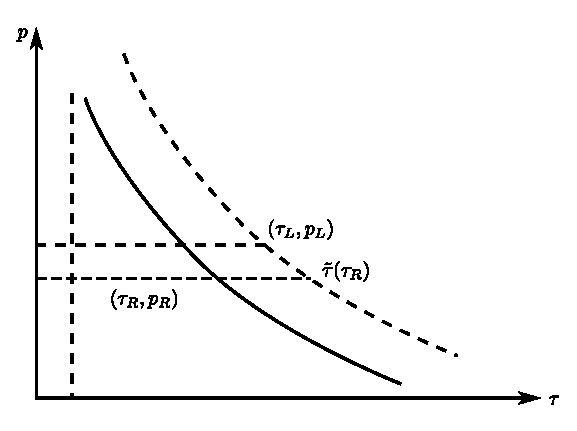
\includegraphics{figures/fig2.4.eps}
\centerline{\bf Fig. 2.4.} 
\end{figure}\pageoriginale
\noindent
most two in between states, each representing states behind $(\tau_R, p_R)$ and $(\tau_L, p_L)$ respectively and connected by a slip or contact discontinuity which appears as the horizontal line $p =$ constant. The velocity $u$ in the two states must be the same. From the right hand side, it is determined either by the shock condition
$$
u = [(p_R - p) \; (\tau - \tau_R)]^{1/2},
$$
using $u_R = 0$ or by the rarefaction formula
$$
u = - \ell_R(\tau_R) + \ell_R(\tau)
$$
and on the left side by
$$
u - u_L = - [(p_L - p) \; (\tau - \tau_L)]^{1/2}
$$\pageoriginale
or
$$
u - u_L = \ell_L (\tau_L) - \ell_L(\tau). 
$$
We note that these formulas are continuous at $\tau = \tau_R$ and $\tau = \tau_L$ respectively. We further note that we connot ``add in'' rarefaction waves or shock waves as part of the states to be connected because we cannot match the velocities.

To solve the Riemann problem we have only to show that we can always find a horizontal segment where the values of $u$ on the intersections with the two $SB$ curves are the same.

But for $p \to \infty$ these intersections correspond to the shock portions of the $SB$ curves, the two values of $\tau$ are approaching their minima and the difference between $u$ on the left $SB$ curve $(\tilde{u}_L)$ and on the right $(\tilde{u}_R)$ satisfies
$$
\tilde{u}_L - \tilde{u}R \to - \infty.
$$
On the other hand as $\tau \to \infty$ a line $p = $ constant intersects the two rarefaction sections of the $SB$ curves. Both $\ell_R(\tau)$ and $\ell_L(\tau) \to 0$ since
$$
\ell = \int\limits^\rho_0 c / \rho d \rho. 
$$
Hence
$$
\tilde{u}_L - \tilde{u}_R \to u_L + \ell_L (\tau_L) + \ell_R(\tau_R). 
$$
Hence if 
$$
u_L + \ell_L  (\tau_L) + \ell_R (\tau_R) > 0
$$
there\pageoriginale is always a solution. On the other hand if
$$
u_L < - \ell_L (\tau_L) - \ell_R (\tau_R) 
$$
we have two completed rarefaction waves and there is a vacuum in between.

Thus every Riemann problem can be solved. The configurations are as follows:

If $u_L$ lies in the interval
$$
[-\ell_L(\tau_L) + \ell_L (\tilde{\tau} (\tau_R)), \; \{(p_R - p (\tilde{\tau}^{-1} (\tau_L)) \; (\tilde{\tau}^{-1} (\tau_L) - \tau_R)\}^{1/2}]
$$
we have a rarefaction from the left and a shock from the right. This includes the case $u_L < 0$ since $\tilde{\tau}(\tau_R) < \tau_L$. If $u_L$ lies in 
$$
[-\ell_L(\tau_L) - \ell_R (\tau_R), \; \ell_L(\tilde{\tau}(\tau_R)) - \ell_L(\tau_L)] 
$$
we have two rarefactions possibly with a vacuum and if 
$$
u_L > \{(p_R - p (\tilde{\tau}^{-1} (\tau_L))) \; (\tilde{\tau}^{-1} (\tau_L) - \tau_R)\}^{1/2} 
$$
there are two shocks.

It is also quite easy to show that $d(\tilde{u}_L - \tilde{u}_R) >0$ provided the Hugoniot curves are star-shaped, which shows that within the class of fan waves our solution is unique.

However, full uniqueness follows only by using a contraction theorem, see, for example, Oleinik \cite{key34} or Keyfitz \cite{key20}.

\section{Solution of initial value problem}\label{chap2:sec2.9}
It was\pageoriginale originally proposed by Godunov that the initial value problem (IVP) should be solved approximately by considering the initial data as approximately piecewise constant and then solving a set of Riemann problems, each by what we shall call a fan solution.
\begin{figure}[H]
\centering
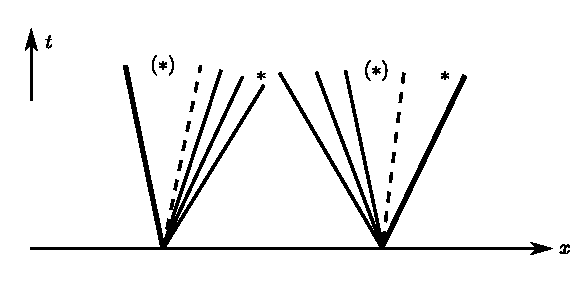
\includegraphics{figures/fig2.5.eps}
\centerline{\bf Fig. 2.5.}
\end{figure}

This solution is considered up to time $\Delta t$ where $\Delta t / \Delta x < 1/2 S$ where $S$ is the maximum of shock speeds or characteristic speeds that occur. This cuts out intersections. At the next time $t$ we have to replace the resulting data again by a piecewise constant solution. It turns out that we must choose this value and place it at $*$ and it must be chosen as the state values at a random point between the $(*)'s$ (See Fig. 2.5). Alternatively (Liu) the values at a point that sweeps out the interval regularly will do.

We assume this set up and state the theorem, show what actually happens in some special cases but first a few summary remarks.

The approach is based on Lax \cite{key23}. We are looking for a weak solution of 
\begin{equation*}
u_t + (F(u))_x = 0 \tag{2.30}\label{eq2.30}
\end{equation*}\pageoriginale
satisfying an entropy condition (stated below). Here $u$ is an $n$ -vector and $F$ is a vector valued function. We assume this system is hyperbolic, i.e., the matrix $F'(u)$ has $n$ real and distinct eigenvalues for all $u$ in some relevant domain. We arrange these eigenvalues, $\lambda_k(u)$, in increasing order
\begin{equation*}
\lambda_1 < \lambda_2 < \ldots < \lambda_n .
\tag{2.31}\label{eq2.31}
\end{equation*}
We also assume the system (\ref{eq2.30}) is genuinely nonlinear in a sense to be chosen. A weak solution of (\ref{eq2.36}) means a bounded measurable function $u$ such that
\begin{equation*}
\int(\chi_t u + \chi_x F(u)) dx = 0\tag{2.32a}\label{eq2.32a}
\end{equation*}
for $\chi \in C^\infty_0$ and a weak solution with initial value $u(x,0) = \phi (x)$ means a weak solution satisfying
\begin{equation*}
\int\limits_{t > 0} (\chi_t u + \chi_x F(u)) dx + \int \chi (x,0) \phi (x) dx = 0
\tag{2.32b}\label{eq2.32b}
\end{equation*}
for all smooth vectors $\chi$ vanishing for large $|x| + t$. A piecewise continuous solution is a weak piecewise continuous solution and hence satisfies the jump condition across a discontinuity:
\begin{equation*}
S[u_K] = [F_k], \; k = 1,2, \ldots ,n,\tag{2.33}\label{eq2.33}
\end{equation*}
where $S$ is the speed of propagation of discontinuity and $[\cdot]$ denotes the jump across the discontinuity.

We now formulate an entropy condition by requiring the following to hold: For some $k$, $l \leq k \leq n$,
\begin{equation*}
\left. 
\begin{aligned}
& \qquad \lambda_k (u_\ell) > S > \lambda_k (u_r) \\
\text{while  }& \\
& \qquad \lambda_{k-1} (u_\ell) < S < \lambda_{k+1} (u_r) \quad 
\end{aligned}
\right\} \tag{2.34}\label{eq2.34}
\end{equation*}\pageoriginale
Here $u_\ell$ and $u_r$ are the states to the left and right of the discontinuity respectively. The eigenvalues $\lambda_k's$ are also called characteristic speeds. The condition (\ref{eq2.34}) says the $k^{\rm th}$ characteristic meets the discontinuity from the left and the $n-(k-1)$ characteristic from the right, the total being equal to $(n+1)$ and thus $(n+1)$ quantities will determine $(2n)$ unknowns and the `shock speed'. This agrees with gas dynamics and combustion.

A discontinuity across which (\ref{eq2.33}) and (\ref{eq2.34}) hold is called a $k-$th shock and $S$ will be called a shock speed.

Suppose for some $k$, $1 \leq k \leq n$, $\grad_u \lambda_k \neq 0$ and is {\em not} orthogonal to $r_k$ the corresponding eigenvector. If this is so, we say $k^{\rm th}$ fan is {\em genuinely nonlinear}. We normalise $r_k$ so that
\begin{equation*}
r_k \cdot \grad_u \lambda_k = 1.  \tag{2.35}\label{eq2.35}
\end{equation*}
If on the otherhand $r_k \cdot \grad_u \lambda_k= 0$ we say the $k^{\rm th}$ fan is {\em linearly degenerate}.

We consider an example from gas dynamics. The equations read (See (\ref{eq2.9a}))
\begin{align*}
& p_t + up_x + \rho c^2 u_x = 0\\
& \rho u_t + p_x + \rho u u_x = 0\\
& S_t + S_x u = 0.
\end{align*}
Here\pageoriginale the matrix $F'(u)$ is given by
$$
\begin{pmatrix}
u & \rho c^2 & 0\\
\rho^{-1} & u & 0\\
0 &  0 &  u
\end{pmatrix}
$$
and $\lambda = u$ is an eigenvalue and the corresponding eigenvector is given by 
$$
\begin{pmatrix}
0\\0\\u_3
\end{pmatrix}
$$
where $u_3 \neq 0$ is arbitrary. Thus the characteristic field corresponding to this eigenvalue is linearly degenerate. (This actually leads to special difficulties in computation, see, e.g., Harten \cite{key17}).

We now state the main result.

\begin{thm}\label{chap2:thm1}
The set of states $u_r$ which are connected to $u_\ell$ for $|u_r - u_\ell|$ sufficiently small through a $k$ - shock from a smooth one parameter family $u_r = u (\epsilon)$, $- \epsilon_o < \epsilon \leq 0$, $u(0) = u_\ell$; the shock speed is also a smooth function of $\epsilon$.
\end{thm}

\begin{remark*}
The entropy condition gives the one sided interval.

We now turn to an important class of solutions, centred rarefaction waves; these are the solutions which depend only on the ratio $(x-x_o)/ (t-t_o)$, $x_o$, $t_o$ are the centre of the wave.
\end{remark*}

Let $u$ be a rarefaction wave centred at the origin:
\begin{equation*}
u(x,t) = h (x/t).\tag{2.36}\label{eq2.36}
\end{equation*}
Substituting\pageoriginale this in (\ref{eq2.36}), we see that
\begin{equation*}
-\frac{x}{t} h' + \frac{1}{t} F' (u) h' = 0 
\tag{2.37}\label{eq2.37}
\end{equation*}
where $'$ denotes differentiation with respect to $\xi = x/t$. Thus $\xi = \lambda_k$ is an eigenvalue of $F'(u)$ and $h'$ is a corresponding eigenvector; $h$ is called a $k$ - {\em rarefaction wave}.

in view of (\ref{eq2.35}), we can take 
\begin{equation*}
h' = r(h).\tag{2.38}\label{eq2.38}
\end{equation*}
Put $\lambda = \lambda (u_\ell)$; (\ref{eq2.38}) has a unique solution satisfying the initial condition
\begin{equation*}
h(\lambda) = u_\ell;
\tag{2.39}\label{eq2.39}
\end{equation*}
$h$ is defined for all $\xi$ close enough to $\lambda$.

Let $\epsilon \geq 0$ be such that $h$ is defined for $\lambda + \epsilon$; write $u_r = h (\lambda + \epsilon)$.

We now construct the following piecewise smooth function $u(x,t)$ for $t \geq 0$ 
(See Figure 2.6).
\begin{equation*}
u(x,t) = 
\begin{cases}
u_\ell \quad \text{for} \quad x < \lambda t\\
h(x/t) \quad \text{for} \quad  \lambda t \leq x \leq (\lambda + \epsilon) t \\
u_r \quad \text{for} \quad (\lambda + \epsilon) t ,x.
\end{cases}
\tag{2.40}\label{eq2.40}
\end{equation*}

\begin{figure}[H]
\centering
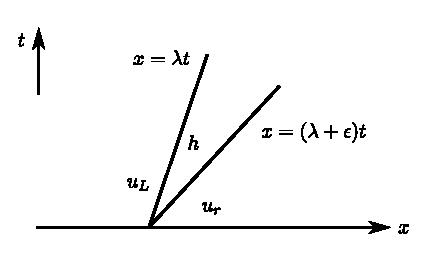
\includegraphics{figures/fig2.6.eps}
\centerline{\bf Fig. 2.6.}
\end{figure}

This function\pageoriginale $u$ satisfies the differential equation (\ref{eq2.36}) in each of three regions, and is continuous across the lines separating the regions. We shall say that in $u$ the states $u_\ell$ and $u_r$ are connected by a centred $k$ - rarefaction wave.

\begin{thm}\label{chap2:thm2}
There exists to every state $u_\ell$ a one parameter family of states $u_r = u(\epsilon)$, $0 \leq \epsilon < \epsilon_o$, connected to $u_\ell$ by a $k$ - rarefaction wave.

We now turn to another important problem, Riemann problem, in which the initial value given are
\begin{align*}
u & = u_o \quad \text{for} \quad x < 0\\
u & = u_1 \quad \text{for} \quad x > 0.
\end{align*}
\end{thm}

\begin{thm}\label{chap2:thm3}
There always exists a solution (a fan wave) to the Riemann problem if $|u_0 - u_1|$ is sufficiently small.

The proof uses only the implicit function theorem and we refer to Lax \cite{key23}.
\end{thm}

\medskip
\noindent{\textbf{Norms: }}
What can we expect: $u_x \in L^1$, not $L^2$, at best since $u$ has jump discontinuities. This suggests looking for a solution $u$ of bounded variation.

We now state a theorem due to Glimm and for the proof we refer to Glimm \cite{key15}. 

\begin{thm}[Glimm]\label{chap2:thm4}
Let  (\ref{eq2.30}) be hyperbolic, strictly (genuinely) nonlinear and $F$ be smooth in a neighbourhood of $u = \tilde{v}$, a constant vector. Then there is a $K < \infty$ and a $\delta > 0$ with the following property:

If the\pageoriginale initial values $u(x,0)$ are given so that\footnote{T.V. = Total variation}
$$
d_1 = || u(., 0) - \tilde{v} ||_\infty + T.V. u(., 0) < \delta,
$$
then there exists a weak solution of (\ref{eq2.36}) for all $x, t \geq 0$ with initial values $u(x,0)$ such that
\begin{align*}
& ||u-\tilde{v}||_\infty \leq K ||u(.,0) - \tilde{v}||_\infty \tag{2.41a}\label{eq2.41a}\\
& T.V. \; u (., t) \leq K (T.V. u (., 0)), \; t \geq 0 \tag{2.41b}\label{eq2.41b}\\
 \int\limits^{+\infty}_{-\infty}  |u(x,t_1) &  - u (x,t_2)| dx \leq K | t_1 - t_2| (T.V. u (.,0)) \tag{2.41c}\label{eq2.41c}
 \end{align*}

For a restricted class including gas dynamics and if 
$$
|| u(.,0) - \tilde{v}||_\infty (1 + T.V. u (.,0)) \leq \delta
$$
then there exists a solution satisfying (\ref{eq2.41a}) and (\ref{eq2.41b}).
\end{thm}

We now describe an approximate method developed by Glim to solve any initial value problem $u(x,0) = u_o (x)$ when the oscillation of $u_o(x)$ is small. The solution $u$ is obtained as the limit of approximate solutions $u_h$, as $h\to 0$, which are constructed as follows:
\begin{itemize}
\item[{\rm (I)}] $u_h (x,0)$ is a piecewise constant approximation to $u_o(x)$
\begin{equation*}
u_h (x,0) = m_j \quad \text{for} \quad jh < x < (j+1)h, \; j = 0, \pm 1, \ldots, \tag{2.42}\label{eq2.42}
\end{equation*}
where $m_j$ is some kind of mean value of $u_o(x)$ in the interval $(jh, (j+1)h)$.

\item[{\rm (II)}] For $0\leq t < h/\lambda$, $u_h(x,t)$ is the exact solution of (\ref{eq2.30}) with initial values $u(x,0)$ given by (\ref{eq2.42}); here $\lambda$ is an upper\pageoriginale bound for $2|\lambda_k(u)|$. This exact solution is constructed by solving the Riemann IVP's,
\begin{equation*}
u(x,0) = 
\begin{cases}
m_{j-1} \quad \text{for} \quad x < jh,\\
m_j \quad \text{for} \quad jh , x,
\end{cases}
\tag{2.43}\label{eq2.43}
\end{equation*}
$j = 0, \pm 1, \ldots$. Since the oscillation of $u_o$ is small, $m_{j-1}$ and $m_j$ are close and so by Theorem \ref{chap2:thm3}, this IVP has a solution consisting of constant states separated by shocks or rarefaction waves issuing from the points $x= jh$, $t=0$ (See Figure 2.7). As long as 
\begin{equation*}
t <  h /\lambda\tag{2.44}\label{eq2.44}
\end{equation*}
these waves do not intersect each other and so the solutions of the IVP (\ref{eq2.43}) can be combined into a single exact solution $u_h$.
\begin{figure}[H]
\centering
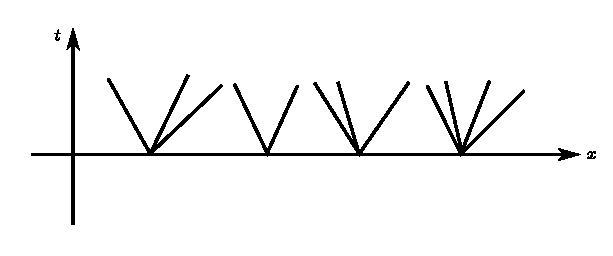
\includegraphics{figures/fig2.7.eps}
\centerline{\bf Fig. 2.7.}
\end{figure}

\item[{\rm (III)}] We repeat the process, with $t = h/\lambda$ as new initial time in place of $t=0$.

It is not at all obvious that this process yields an approximate solution $u_h$ which is defined for all $t$; to prove\pageoriginale this one must show that the oscillation of $u(x,nh)$ remains small, uniformly for $n = 1,2, \ldots$ and so that one can solve Riemann IVPs (\ref{eq2.43}). This estimate turns out to depend very sensitively on the kind of average used to compute the mean values $m_j$. Glimm has used the following method to compute $m_j$:

A sequence of random numbers $\alpha_1 , \alpha_2, \ldots$ {\em uniformly distributed} in $[0,1]$ is chosen; $m^n_j$ then mean value of $u(x, nh/\lambda)$ over the interval $(jh, (j+1)h)$ is taken to be 
\begin{equation*}
m^n_j = u (jh + \alpha_nh, \; nh /\lambda). 
\tag{2.45}\label{eq2.45}
\end{equation*}
Glimm proves the following.
\end{itemize}

\begin{thm}\label{chap2:thm5}
A subsequence of $u_h$ converges in $L^1$ with respect to $x$, to a weak solution of (\ref{eq2.30}), uniformly in $t$, and for almost all choices of $\{\alpha_n\}$.
\end{thm}

For the proof we refer to Glimm \cite{key15} and we illustrate here by an example; see Lax \cite{key23}.

Consider a Riemann IVP
$$
u(x,0) = 
\begin{cases}
& u_\ell \quad \text{for} \quad x < 0\\
& u_r \quad \text{for} \quad x > 0
\end{cases}
$$
where $u_\ell$ and $u_r$ are so chosen that the exact solution $u$ consists of the two states $u_\ell$, $u_r$ separated by  a shock,
\begin{equation*}
u(x,t) = 
\begin{cases}
u_\ell \quad \text{if} \quad x < st,\\
u_r \quad \text{if} \quad x > st,
\end{cases}
\tag{2.46}\label{eq2.46}
\end{equation*}
where\pageoriginale $s$ is the shock speed. We may take $\lambda >|s|$. Assume $s>0$. Glimm's recipe gives
$$
u_h (x,h/\lambda) =
\begin{cases}
u_\ell \quad \text{if} \quad x < J_1 h\\
u_r \quad \text{if} \quad J_1 h < x
\end{cases}
$$
where
$$
J_1 = 
\begin{cases}
1 \quad \text{if} \quad  \alpha_1 < s/ \lambda\\
0 \quad \text{if} \quad s /\lambda < \alpha_1
\end{cases}
$$
Repeating this procedure $n$ times, we obtain
$$ 
u_h(x, nh/\lambda) =
\begin{cases}
u_\ell \quad \text{for} \quad x < J_nh,\\
u_r \quad \text{for} \quad J_nh < x,
\end{cases}
$$
where $J_n = $ number of $\alpha_j's$, $j = 1,2,\ldots, n$, such that $\alpha_j , s / \lambda$. Since $\{\alpha_j\}$ is a uniformly distributed random sequence in $[0,1]$
$$
\frac{J_n}{n} \to \frac{s}{\lambda}
$$
with probability $1$; this tells the approximate solution tends almost surely to the exact solution.

One would like to prove more about the solution of the initial value problem. In particular the uniqueness of the solution. Some results are contained in DiPerna \cite{key8} but they are not applicable to the general initial value problem because they do not admit shock formations within the flow.

\section{Combustion. Detonations and deflagrations}\label{chap2:sec2.10}
In this\pageoriginale section, we present a brief account of the elementary theory of detonation and deflagration waves. These differ from shocks as the increased pressure releases energy and converts one gas into another in a chemical reaction. We denote this energy, per unit mass, the energy of formation, by $g$ and the total energy
$$
E = e+ g
$$
where $e$ is internal energy. In this case the equations of the gas dynamic are
\begin{gather*}
\rho_t + (\rho u)_x = 0\\
(\rho u)_t + (\rho u^2 +p)_x = 0,\tag{2.47}\label{eq2.47}\\
\tilde{E}_t + ((\tilde{E} + p)u)_x = 0,
\end{gather*}
where $\rho$ is the density, $u$ is the velocity, $p$ is the gas pressure. But $\tilde{E}$ depends on the precise nature of the gas and is given by
$$
\tilde{E} = \rho E + \rho u^2 / 2.
$$

Let the subscript $0$ refer to unburnt gas and $1$ to burnt gas. Let the unburnt gas be to the right of the reaction zone and let $U$ be the velocity of the reaction zone. Then the two laws of conservation of mass and momentum are identical with the corresponding laws for shock fronts and we have 
\begin{align*}
& \rho_o v_o = \rho_1 v_1 = m, \tag{2.48}\label{eq2.48}\\
& p_o + \rho_o v^2_o = p_1 + \rho_1 v^2_1 \tag{2.49}\label{eq2.49}
\end{align*}\pageoriginale
where $v_i = u_i - U$, $i = 0,1$, are the relative velocities. The law of conservation of energy now takes the form:
\begin{equation*}
E^{(o)} (\tau_o, p_o) + p_o \tau_o + v^2_o / 2 = E^{(1)} (\tau_1, p_1) + p_1 \tau_1 + v^2 _1 / 2 \tag{2.50}\label{eq2.50}
\end{equation*}
where $E^{(1)}$ and $E^{(o)}$ are two different energy functions. As in the case of shock fronts we consider  the Hugoniot function
$$
H(\tau_1, p_1 ; \tau_o , p_o) = E^{(1)} (\tau_1, p_1) - E^{(o)} (\tau_o, p_o) + (\tau_1 - \tau_o) (p_1 + p_o) / 2.
$$
It should be stressed that the conservation of energy (\ref{eq2.50}) is entirely different from that in the case of shock fronts but that any law derived from the conservation of  mass and momentum still holds.

Using (\ref{eq2.48}) and (\ref{eq2.49}), (\ref{eq2.50}) can be written as
\begin{equation*}
H(\tau_1, p_1 ; \tau_o , p_o) = 0.\tag{2.51}\label{eq2.51}
\end{equation*}
As in the previous case, the graph of $(\tau_1, p_1)$ in the $(\tau, p)$ plane, which satisfies (\ref{eq2.51}) for fixed $(\tau_o, p_o)$ will be called the {\em Hugoniot curve with center $(\tau_o, p_o)$.} For polytropic gases, we have
$$
e = \frac{p\tau}{\gamma -1}, \quad \gamma \geq 1.
$$
If we set $\Delta =g_o - g_1$ ($\Delta \leq 0$ for an exothermic process) and $\mu^2 = \dfrac{\gamma -1}{\gamma +1}$, we find 
\begin{equation*}
0 = 2\mu^2 H = -p_o (\tau_o - \mu^2 \tau_1) + p_1 (\tau_1 - \mu^2 \tau_o) - 2 \mu^2 \Delta . \tag{2.52}\label{eq2.52}
\end{equation*}
As in\pageoriginale the previous case, this is a rectangular hyperbola. This time the point $(\tau_o, p_o)$ does not lie on the hyperbola because of the extra term due to $\Delta$. In fact, if $\Delta \leq 0$, $(\tau_o, p_o)$ lies below the Hugoniot curve; see figure 2.8. We assume this in general.

The lines through $(\tau_o, p_o)$ tangent to $H=0$ are called {\em Rayleigh lines}. Their points of tangency, $S_1$ and $S_2$, are called {\em Chapman-Jouguet (CH) points}. The portion $p> p_o$, $\tau > \tau_o$, of the Hugoniot curve is omitted because it corresponds to the impossible case in which $m^2 < 0$. Here we have used the relation
$$
-m^2 = \frac{p_o - p_1}{\tau_o - \tau_1},
$$
which follows from (\ref{eq2.48}) and (\ref{eq2.49}). The upper portion of the Hugoniot curve corresponds to {\em detonations} (increase in pressure); the portion above $S_1$ corresponds to strong detonations and below $S_1$ to weak detonations. The lower portion of the Hugoniot curve corresponds to deflagrations (decreases in pressure). These two pieces might appear to be playing the role of a ``state behind'' curve and we might anticipate that shocks and detonations are linked while deflagrations and simple waves are related. However, considerations of the internal mechanism appears to eliminate deflagrations and weak detonations except in special cases.

The relative speeds of fronts governed by the Hugoniot curve can be determined by differentiation.
\begin{figure}[H]
\centering
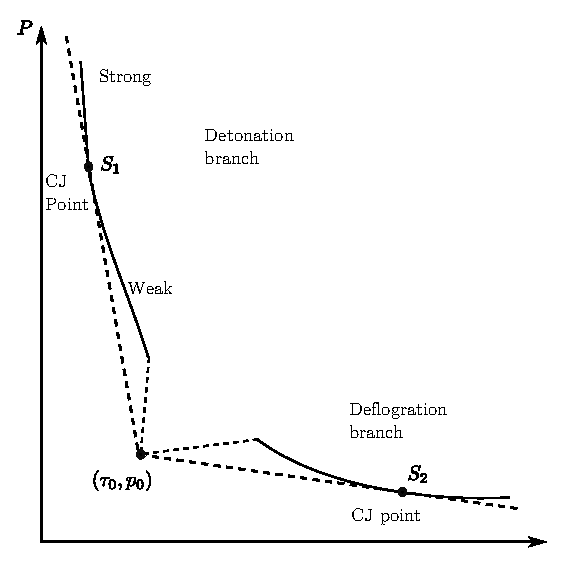
\includegraphics{figures/fig2.8.eps}
\centerline{{\bf Fig. 2.8.} The Hugoniot curve for exothermic gas flow}
\end{figure}\pageoriginale

First of all,
$$
0 = dH (\tau, p) = TdS + \frac{1}{2} \{ (\tau - \tau_o)d p+ (p-p_o) d\tau\}.
$$
Thus for a Chapman-Jouguet process where $(\tau-\tau_o) dp+ (p-p_o) d\tau = 0$ we have $dS =0$. So at this point
$$
\frac{p-p_o}{\tau-\tau_o} = \frac{dp}{d\tau} = \frac{\partial p}{\partial \tau} \mid_1 = -\frac{1}{\tau^2_1} c^2_1. 
$$
Thus by the mechanical conditions
$$
v^2_1 = -\tau^2 _1 (p-p_o) / (\tau - \tau_o) = c^2 _1.
$$
That is, the state behind is sonic relative to the front. On the other hand
$$
v^2_o =- \tau^2_o (p-p_o) / (\tau - \tau_o)
$$ 
and along the Hugoniot curve
$$
dv^2_1 = \tau^2_o ((p-p_o) d\tau - (\tau-\tau_o)dp)
$$\pageoriginale
so that $v_o$ has stationary value for a Chapman-Jouguet process and furthermore it is a minimum. Hence the flow ahead of a strong or weak detonation is supersonic and of a strong or weak deflagration is subsonic provided the Hugoniot curve has the usual convexity.

By looking at the Hugoniot curve for the state behind in a similar way
we find that $v^2_1$ is monotonic on each branch. Hence the flow is
supersonic behind a weak detonation, subsonic hebind a strong
detonation, supersonic behind a strong deflagration and subsonic
behind a weak deflagration. See Fig. 2.9.

\newpage


\begin{figure}[H]
\centering
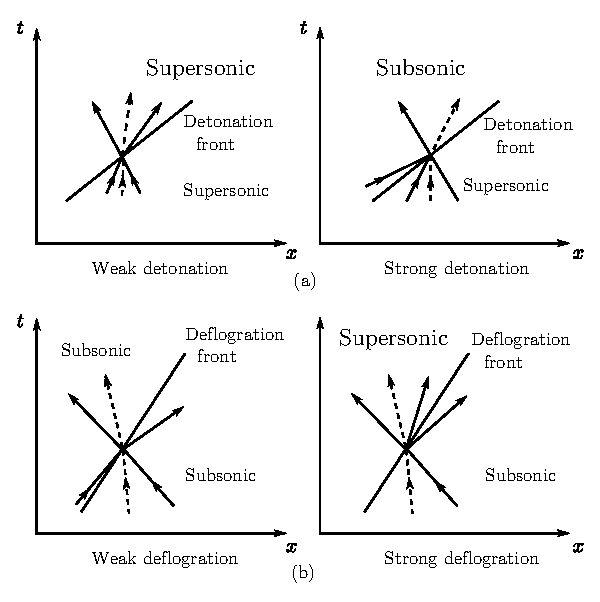
\includegraphics{figures/fig2.9.eps}
\centerline{\bf Fig. 2.9.}
\end{figure}


This\pageoriginale leads to Figure 2.9 which shows the way the three characteristics can leave and enter a front. Each characteristic is carrying one datum. Thus for a strong detonation, one piece of data must be given along with the state in front and the two remaining quantities are then determined. See the corresponding shock wave problem.

\section{Riemann problem with detonations and deflagrations}\label{chap2:sec2.11}

We assume there are only two gases, burnt and unburnt, and that the unburnt gas is on the right with $u_R = 0$. Then there are the following possibilities:

\textit{To the right of the contact discontinuity or slip line either }
\begin{itemize}
\item[{\rm a)}] \textit{a strong detonation or}

\item[{\rm b)}] \textit{a $CJ$ detonation followed by a rarefaction wave or}

\item[{\rm c)}] \textit{a rarefaction wave}
\end{itemize}
\textit{and on the left either a shock or a rarefaction.}

This includes the unlikely case (c) when the pressure in the unburnt gas $p_R$ exceeds that in the burnt $p_L$. Weak detonations and all deflagrations have been eliminated for other reasons to be discussed later.

The $SB$ curve for the left state is the same in section \ref{chap2:sec2.8}. The $SB$ curve for the right state row consists  of the strong detonation branch connected at the Chapman-Jouguet point to an adiabatic curve $p = p(\tau)$ and there is also the rarefaction curve through $p_R$ for use in case (c).

Exactly\pageoriginale the same kind of argument then shows the Riemann problem for the case $p_R < p_L$ can be used again, i.e., connecting the two continuous curves by a line segment and matching up the values of $u$ which are given by the same formulas unless there is a $C-J$ detonation when 
$$
\tilde{u}_R = c(\tau^*, S^*) - \ell_{CJ} (\tau, S^*) + \ell_{CJ} (\tau^*, S^*),
$$
and $\tilde{u}_L$ as before.

Here, $\tau^*$, $S^*$ are the specific volume and entropy at the Chapman-Jouguet detonation and $\ell_{CJ}$ is the `$\ell$' corresponding to that state.

The originale shock wave argument continues to work for $p_R >p_L$ if a shock or rarefaction on the left and a rarefaction on the right are generated. The excluded case is the two-shock case because the unburnt gas is detonated. For 
$$
u_L < [(p_L - p(\tilde{\tau} (T_R))) (\tilde{\tau}(\tau_R) - \tau_L)]^{1/2}
$$
there will be a solution without detonations. If $u_L$ does not satisfy this inequality, then there is a detonation. However, uniqueness is lacking.

\section{Internal mechanism}\label{chap2:sec2.12}
We now investigate why only certain processes take place by looking into the internal mechanism of the front. We look for steady state solutions in one dimension where we now assume the flow has viscosity and heat conductivity. Let the temperature be $\theta$. The conservation of mass remains the same as before:
$$
\rho v = \rho_o v_o = m, \text{ a constant.}
$$\pageoriginale
We seek a continuous flow that moves from a constant state at $x = - \infty$ to a constant state at $x = + \infty$. We assume the flow is moving from right (unburnt) to left (burnt) and the reaction front has fixed velocity, so $m>0$, and $x = + \infty$ is ahead, $x = - \infty$ is behind. The conservation of momentum is given by
$$
\rho v^2 + p - \mu \frac{dv}{dx} = p, \text{ a constant,}
$$
where $\mu$ is the coefficient of viscosity.

Next, at any stage the gas has internal energy $E^{(\epsilon)}(\theta)$ and the energy balance is influenced by heat conduction. Denoting by $\lambda$, the coefficient of heat conduction, the energy balance is written as:
$$
-\lambda \frac{d\theta}{dx} + m \{E^{(\epsilon)} (\theta) + \frac{1}{2} v^2\} + v \{p - \mu \frac{dv}{dx}\} = m Q = \text{ constant.}
$$

Following Friedrichs (see \cite{key11}), we assume the balance between burnt and unburnt gases is 
$$
-v\frac{d\epsilon}{dx} + (1-\epsilon) \; S(\theta) = 0,
$$
where we try to avoid specifying too much about $S(\theta)$. So, we have three autonomous equations and they have {\em singular points } exactly at possible end states.

We write $E^{(0)} (\theta_o) = E_o$ and $E^{(1)} (\theta_1) = E_1$ and investigate the singular points and find that at $x = - \infty$ (state `0') there are in general solutions behaving like 
$$
e^{\alpha_1 x}, \; e^{\alpha_2 x}, \; e^{\alpha_3 x},
$$\pageoriginale
where $\alpha_1 > 0$, $\alpha_2 = 0 $ and 
\begin{align*}
& \alpha_3 > 0 \quad \text{if} \quad v_o \geq c_o\\
& \alpha_3 < 0 \quad \text{if} \quad v_o < c_o.
\end{align*}
Here the suffix $0$ corresponds to the unburnt gas and $c_o$ is the sound speed in the unburnt gas.

The manifold of regular solutions (i.e., tending to constant as $x \to - \infty$) has two free parameters if $v_o \geq c_o$ and only one if $v_o < c_o$. Call the number of parameters $\gamma_o$. Analogously, at the other end, we find the manifold of regular solutions has one free parameter if $v_1 > c_1$ and two if $v_1 \leq c_1$; call the number of free parameters $\gamma_1$.

When can we even hope to find a solution going from state (0) to state (1)? We have three quantities to solve for. We must impose $(3-\gamma_o)$ initial conditions to leave the state (0) and $\gamma_1$ parameters characterise regular solution at $+ \infty$. But one is used up by an arbitrary shift in $x$. Hence $(\gamma_1-1)$ parameters are to be chosen subject to $(3-\gamma_o)$ conditions. So we need $\gamma_1 - 1 \geq 3 - \gamma_o$, i.e., $4-\gamma_o - \gamma_1 \leq 0$ or else {\em some other quantity must be specially chosen}. Thus:
\begin{tabbing}
Strong detonation \quad  \= $v_o \geq c_o$, \; $\gamma_o = 2$  \=  \\
\> \> $4 - \gamma_o - \gamma_1 = 0$\\
\>  $v_1 \leq c_1$, \; $\gamma_1 = 2$ \> 
\end{tabbing}
\begin{tabbing}
Weak detonation \quad  \= $v_o \geq c_o$, \; $\gamma_o = 2$  \=  \\
\> \> $4 - \gamma_o - \gamma_1 = 1$\\
\>  $v_1 \geq c_1$, \; $\gamma_1 = 1$ \> 
\end{tabbing}\pageoriginale
\begin{tabbing}
Strong deflagration \quad  \= $v_o \leq c_o$, \; $\gamma_o = 1$  \=  \\
\> \> $4 - \gamma_o - \gamma_1 = 2$\\
\>  $v_1 \geq c_1$, \; $\gamma_1 = 1$ \> 
\end{tabbing}
\begin{tabbing}
Weak deflagration \quad  \= $v_o \leq c_o$, \; $\gamma_o = 1$  \=  \\
\> \> $4 - \gamma_o - \gamma_1 = 1$\\
\>  $v_1 \leq c_1$, \; $\gamma_1 = 2$ \> 
\end{tabbing}

So over determinacy the internal mechanism matches the {\em under} determinacy of the characteristic problem as given in \S\ \ref{chap2:sec2.11}. 

When the topology of the solution curves is worked out, it turns out that
\begin{itemize}
\item[{\rm (i)}] All strong detonations are possible,

\item[{\rm (ii)}] $CJ$ detonations are only possible if one of the parameters satisfies a special condition, 

\item[{\rm (iii)}] Weak detonations are not possible except under very special conditions,

\item[{\rm (iv)}] Weak deflagrations are as in (iii) and 

\item[{\rm (v)}] Strong deflagrations do not exist.
\end{itemize}
